\section{Evaluation} \label{evaluation}

We evaluated Neptune against Julia on a computer with 16 GB RAM, and Intel Core i7-4790 CPU with 8 cores reported to the OS, frequency up to $3.60$~GHz and 32KB, 256KB, 8MB L1, L2, L3 caches respectively.
The processor's hardware frequency governor was set to ``performance'' mode to disable power saving features.
We also excercised the processor before measuring the results for each benchmark to simulate a long-running execution as the CPU frequency governor dials down the frequency when many cores are used for a long time to maintain the temperature.
We used the following benchmarks for evaluation: Building Julia's core image and system image, i.e. compiling the standard library while using type inference engine \emph{written in Julia} (\texttt{coreimg}); Microbenchmarks used for promoting Julia on its website (\texttt{micro}); a matrix concatenation benchmark (\texttt{cat}) since matrix concatenation is used a lot by programmers with MATLAB background which constitute a considerable amount of Julia's user base; Peter Norvig's spellchecker (\texttt{spell}), this benchmark is used in other garbage collection papers such as \cite{marlow2008parallel}; a handwritten benchmark (\texttt{shallow}) that creates lots of garbage in young generation; implementation of Hans Boehm's "An Artificial Garbage Collection Benchmark" in Julia (\texttt{boehm}).

The optimal speedup is observed with 5-6 worker threads (Figure~\ref{fig:speedup}), after that point threads start racing for cores fewer than the threads\footnote{There is 1 additional thread to coordinate the worker threads and the machine was running \texttt{X} and \texttt{ssh} during our benchmarks to simulate a realistic situation.}.
\cite{marlow2011multicore} also observes a similar congestion behaviors.
As seen in the throughput and latency results (Figures~\ref{fig:throughput} and \ref{fig:latency}), our garbage collector has on average ~30\% worse single-threaded performance due to overhead of maintaining thread safety and due to some sweeping work Julia's GC offloads to allocation that we didn't offload to.
Marlow et al. also report similar overhead for GHC's parallel garbage collector \ref{marlow2008parallel}.

\begin{figure}[h]
  \centering
    \begin{subfigure}{0.32\textwidth}
      \centering
      % \vspace{-2em}
      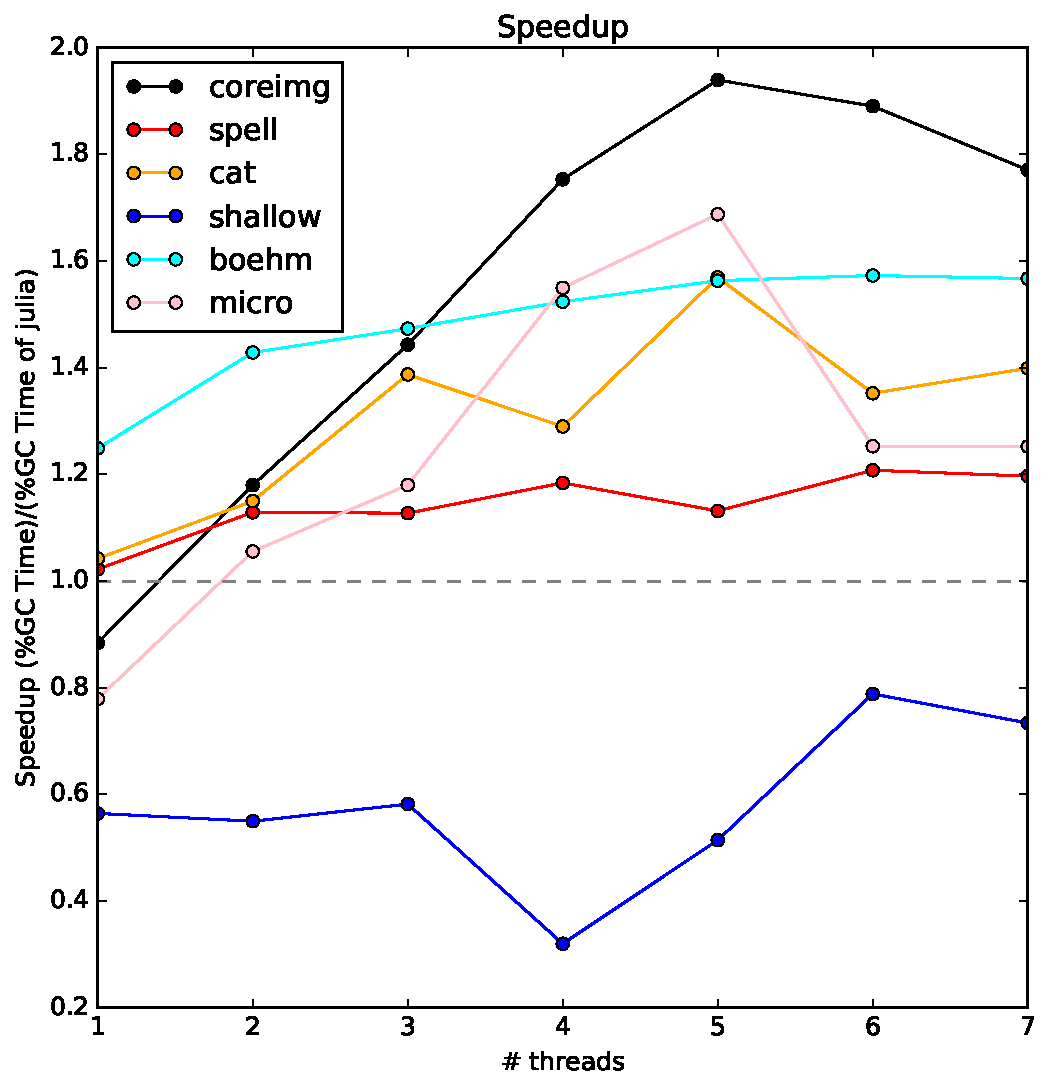
\includegraphics[height=4.8cm]{figures/speedup-julia.pdf}
      \caption{Speedup over Julia}
      \label{fig:speedup}
    \end{subfigure}
    \begin{subfigure}{0.32\textwidth}
      \centering
      % \vspace{-2em}
      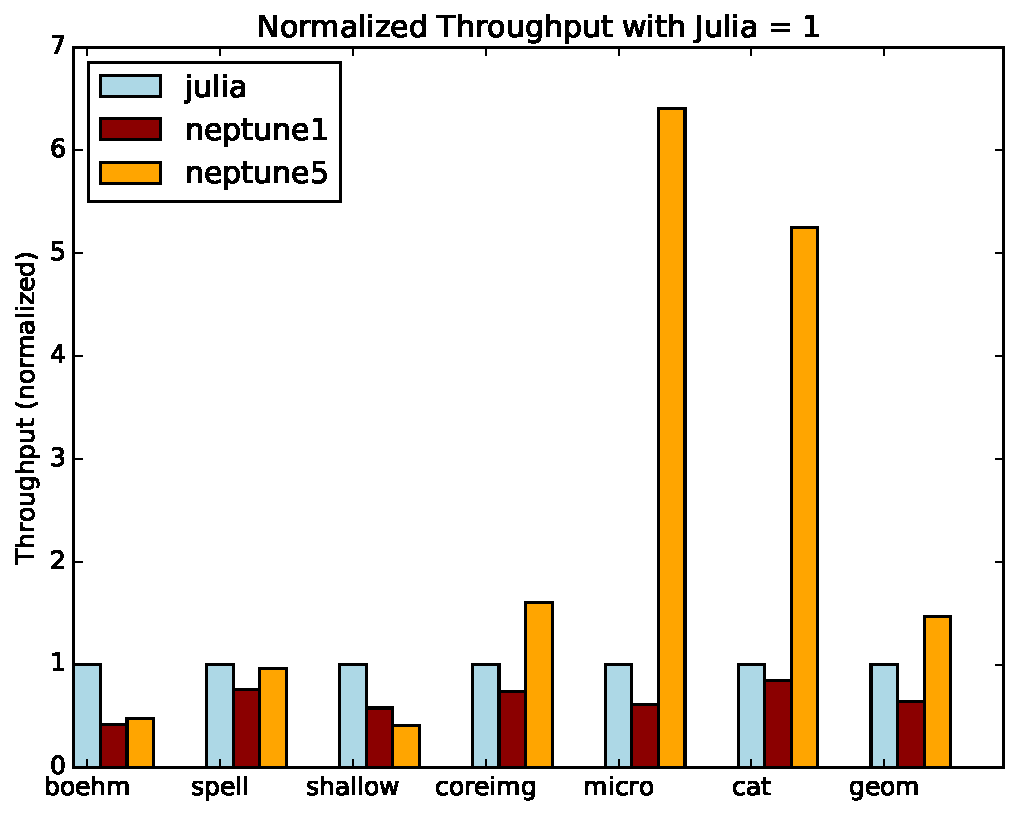
\includegraphics[height=4.8cm]{figures/throughput-normalized-julia.pdf}
      
      \caption{Normalized throughput}
      \label{fig:throughput}
    \end{subfigure}
    \begin{subfigure}{0.32\textwidth}
      \centering
      % \vspace{-2em}
      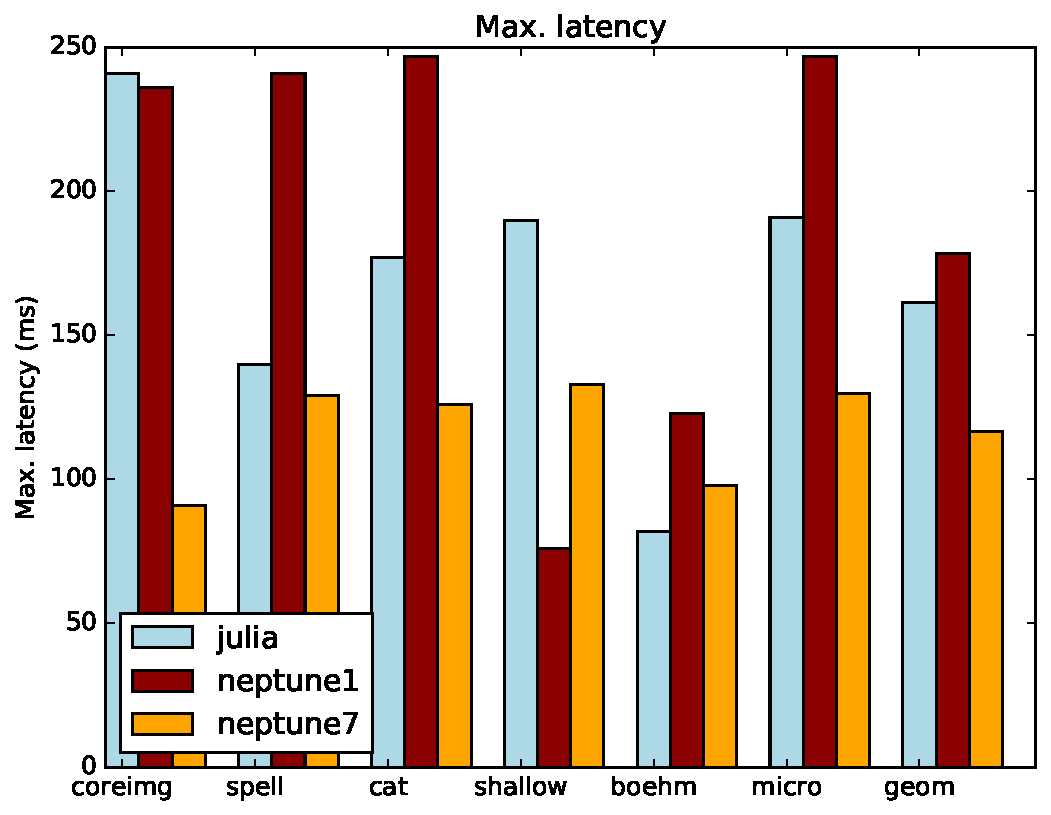
\includegraphics[height=4.8cm]{figures/max-latency.pdf}
      %\todo{FIX neptune7 WITH neptune5}
      \caption{Maximum GC latency (ms)\\}
      \label{fig:latency}
    \end{subfigure}
    \vspace{-0.5em}
    \caption{Experiment results. Figure~\ref{fig:speedup} shows speedup over Julia in terms of \% time taken in GC normalized with Julia = 1. Figure~\ref{fig:throughput} shows throughput normalized with Julia = 1.}
  \label{fig:results}
\end{figure}

%%% Local Variables:
%%% mode: latex
%%% TeX-master: "report"
%%% End:
